\documentclass[journal]{vgtc}                % final (journal style)
%\documentclass[review,journal]{vgtc}         % review (journal style)
%\documentclass[widereview]{vgtc}             % wide-spaced review
%\documentclass[preprint,journal]{vgtc}       % preprint (journal style)
%\documentclass[electronic,journal]{vgtc}     % electronic version, journal

%% Uncomment one of the lines above depending on where your paper is
%% in the conference process. ``review'' and ``widereview'' are for review
%% submission, ``preprint'' is for pre-publication, and the final version
%% doesn't use a specific qualifier. Further, ``electronic'' includes
%% hyperreferences for more convenient online viewing.

%% Please use one of the ``review'' options in combination with the
%% assigned online id (see below) ONLY if your paper uses a double blind
%% review process. Some conferences, like IEEE Vis and InfoVis, have NOT
%% in the past.

%% Please note that the use of figures other than the optional teaser is not permitted on the first page
%% of the journal version.  Figures should begin on the second page and be
%% in CMYK or Grey scale format, otherwise, colour shifting may occur
%% during the printing process.  Papers submitted with figures other than the optional teaser on the
%% first page will be refused.

%% These three lines bring in essential packages: ``mathptmx'' for Type 1
%% typefaces, ``graphicx'' for inclusion of EPS figures. and ``times''
%% for proper handling of the times font family.

\usepackage{mathptmx}
\usepackage{graphicx}
\usepackage{times}
\usepackage{epstopdf}

%% We encourage the use of mathptmx for consistent usage of times font
%% throughout the proceedings. However, if you encounter conflicts
%% with other math-related packages, you may want to disable it.

%% This turns references into clickable hyperlinks.
\usepackage[bookmarks,backref=true,linkcolor=black]{hyperref} %,colorlinks
\hypersetup{
  pdfauthor = {},
  pdftitle = {},
  pdfsubject = {},
  pdfkeywords = {},
  colorlinks=true,
  linkcolor= black,
  citecolor= black,
  pageanchor=true,
  urlcolor = black,
  plainpages = false,
  linktocpage
}

%% If you are submitting a paper to a conference for review with a double
%% blind reviewing process, please replace the value ``0'' below with your
%% OnlineID. Otherwise, you may safely leave it at ``0''.
\onlineid{0}

%% declare the category of your paper, only shown in review mode
\vgtccategory{Research}

%% allow for this line if you want the electronic option to work properly
\vgtcinsertpkg

%% In preprint mode you may define your own headline.
%\preprinttext{To appear in an IEEE VGTC sponsored conference.}

%% Paper title.

\title{Visualizing Data from Massive Online Open Courses}

%% This is how authors are specified in the journal style

%% indicate IEEE Member or Student Member in form indicated below
\author{Katelin Bailey, Jialin Li, Naveen Kr. Sharma}
%\authorfooter{
%%% insert punctuation at end of each item
%\item
% Roy G. Biv is with Starbucks Research. E-mail: roy.g.biv@aol.com.
%\item
% Ed Grimley is with Grimley Widgets, Inc.. E-mail: ed.grimley@aol.com.
%\item
% Martha Stewart is with Martha Stewart Enterprises at Microsoft
% Research. E-mail: martha.stewart@marthastewart.com.
%}

%other entries to be set up for journal
%\shortauthortitle{Biv \MakeLowercase{\textit{et al.}}: Global Illumination for Fun and Profit}
%\shortauthortitle{Firstauthor \MakeLowercase{\textit{et al.}}: Paper Title}

%% Abstract section.
\abstract{This project addresses the massive amount of data available to instructors of 
MOOCs (massive open online courses). While some of the data is noise---students
who never intend to participate, or fail to submit the majority of assignments
---much of it is potentially valuable data on what methods and components in a
course are effective. It is, however, massive in quantity. We intend to use the
data readily available from Coursera to provide some exploratory visualizations
for a generic MOOC class, generally tracking attrition and success rates.

More specifically, we will enable professors, who upload their own data, to add
ress a variety of questions, including but not limited to the following:
(1) Comparing two (or more) instances of the same course: was change X in 
  assignment 3 effective? Were the overall statistics comparable?
(2) Tracking characteristics throughout the course, based on intro 
  demographic information. Do people who don't know recursion do significantly
  worse on this quiz?
(3)racking the timeline of the course: when do people drop out? Can we 
  tell why? 
For the purposes of this project, we will be prototyping from Dan Grossman's 
data, and working with him to determine desirable visualizations.
} % end of abstract

%% Keywords that describe your work. Will show as 'Index Terms' in journal
%% please capitalize first letter and insert punctuation after last keyword
%\keywords{education}

%% ACM Computing Classification System (CCS). 
%% See <http://www.acm.org/class/1998/> for details.
%% The ``\CCScat'' command takes four arguments.

%\CCScatlist{ % not used in journal version
% \CCScat{K.6.1}{Management of Computing and Information Systems}%
%{Project and People Management}{Life Cycle};
% \CCScat{K.7.m}{The Computing Profession}{Miscellaneous}{Ethics}
%}

%% Uncomment below to include a teaser figure.
  \teaser{
  \centering
%  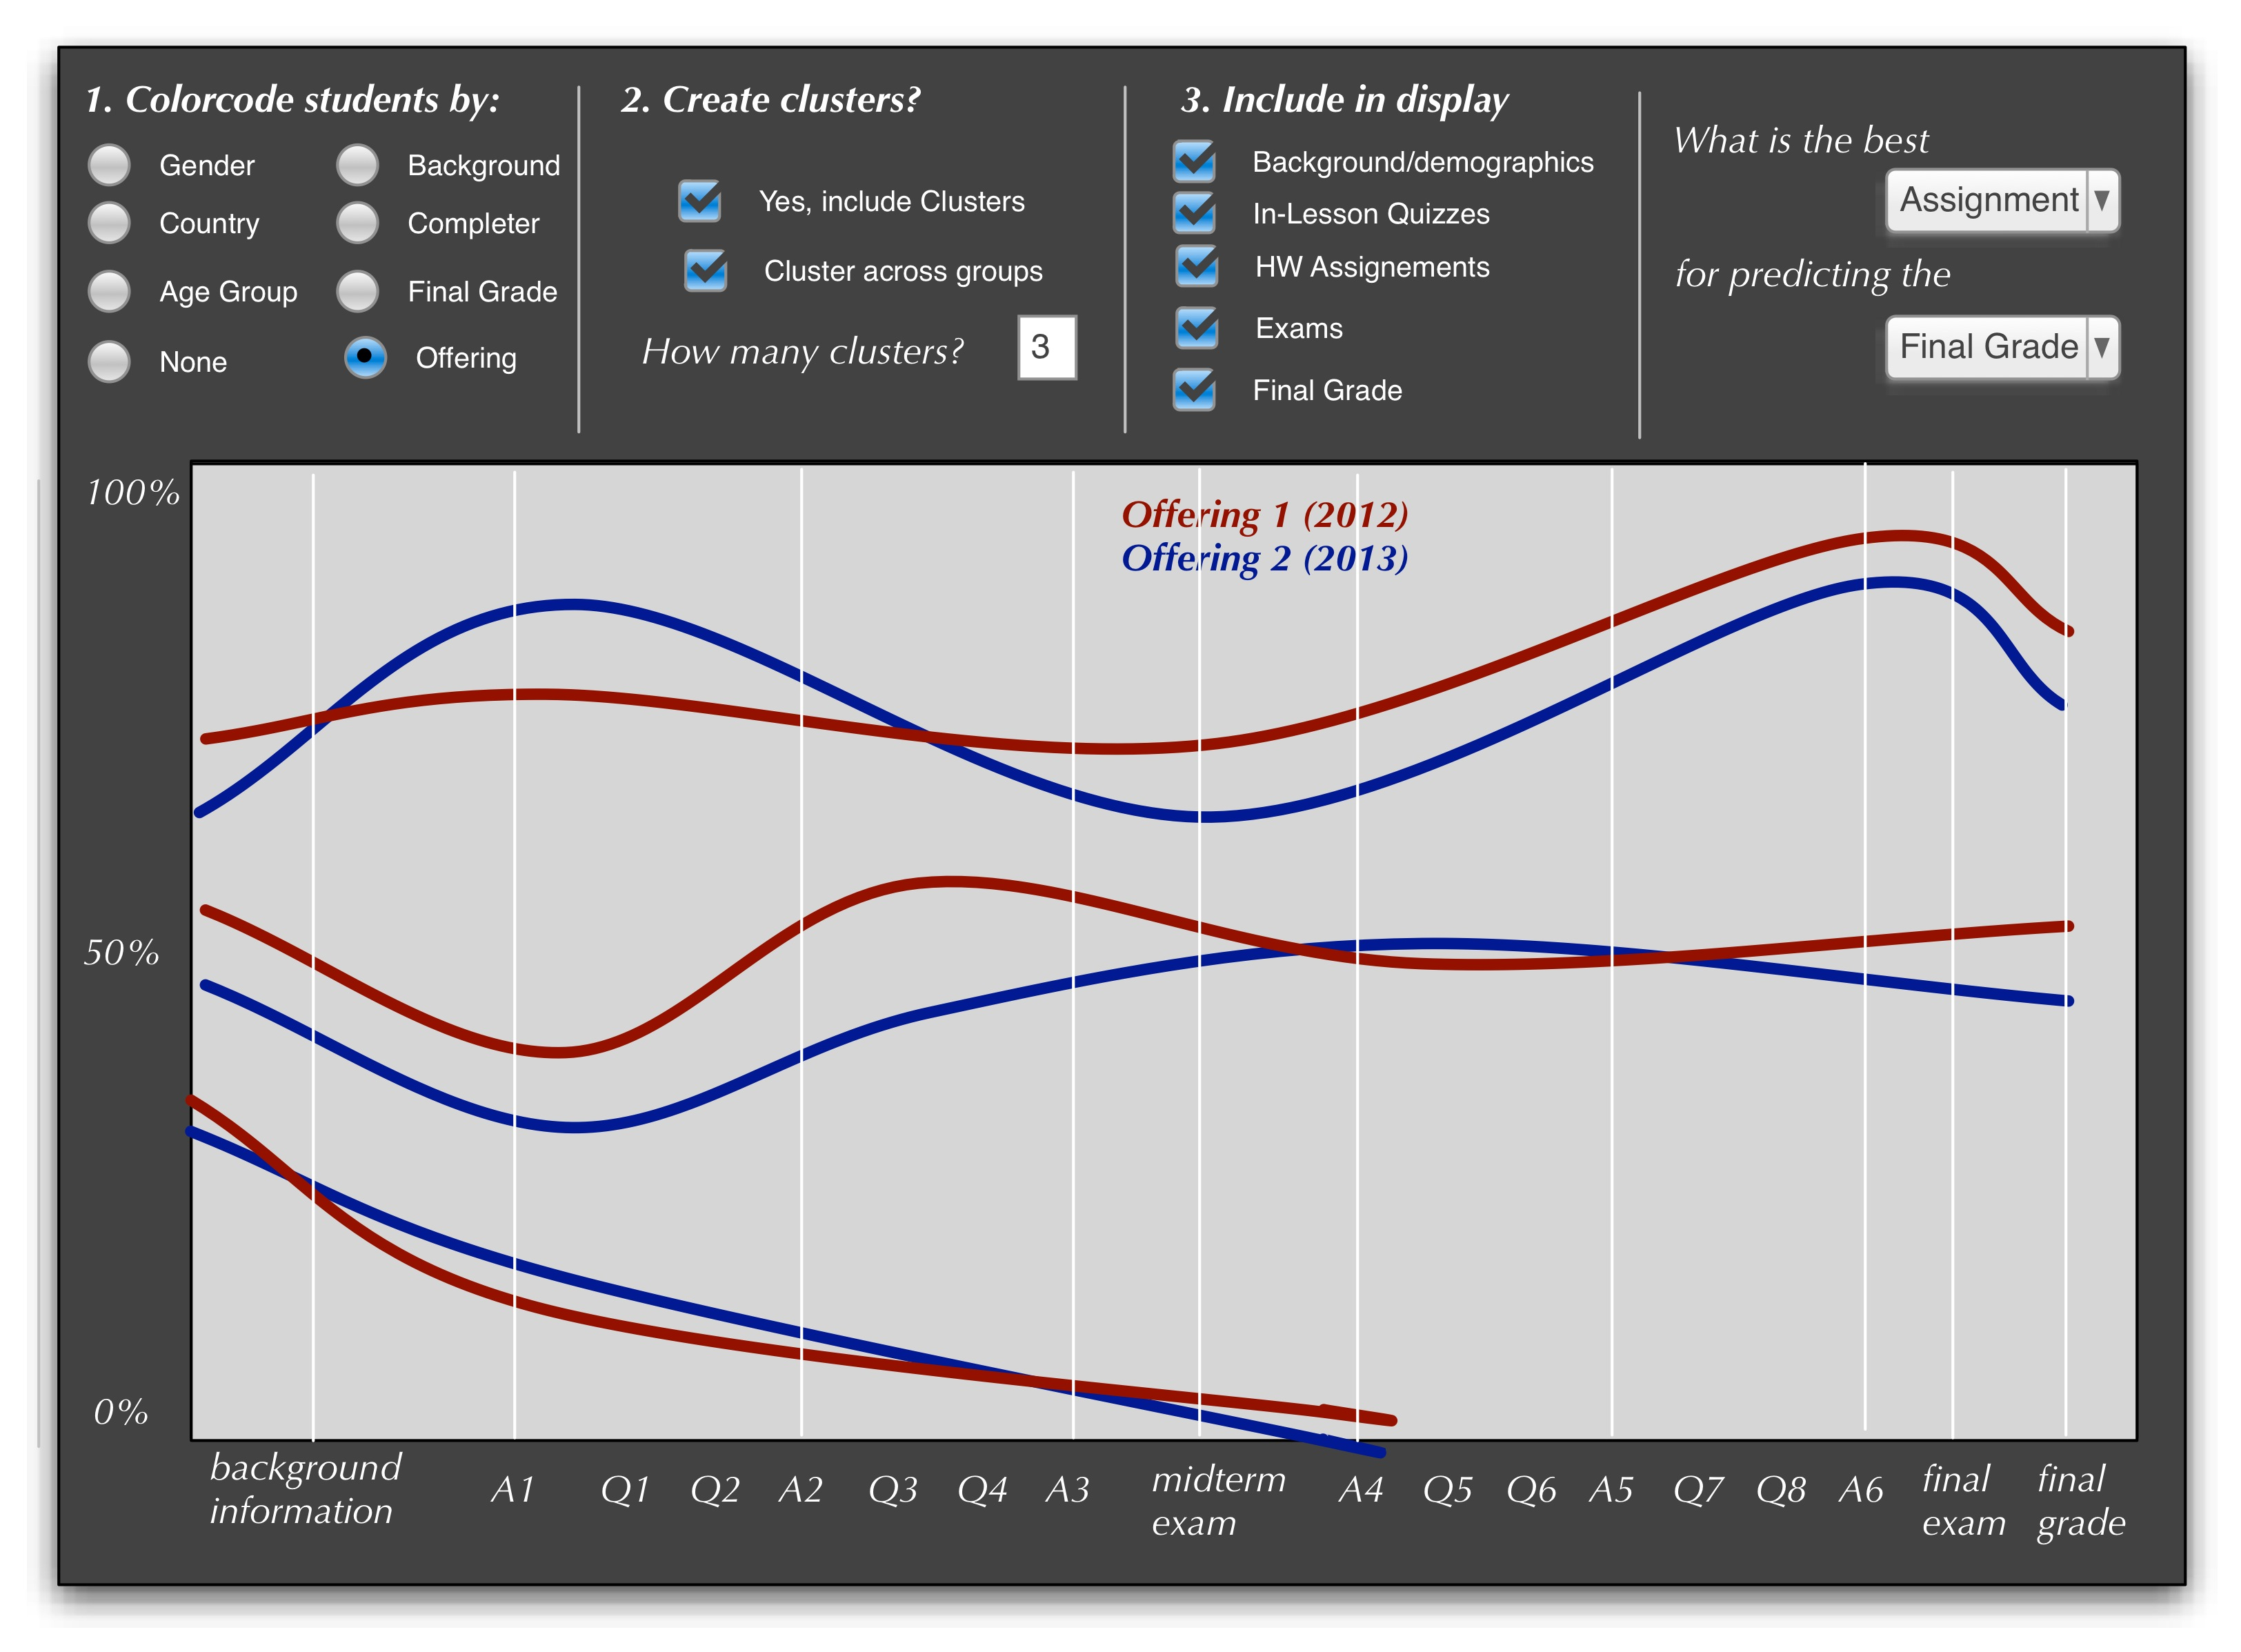
\includegraphics[width=16cm]{storyboard.jpg}
  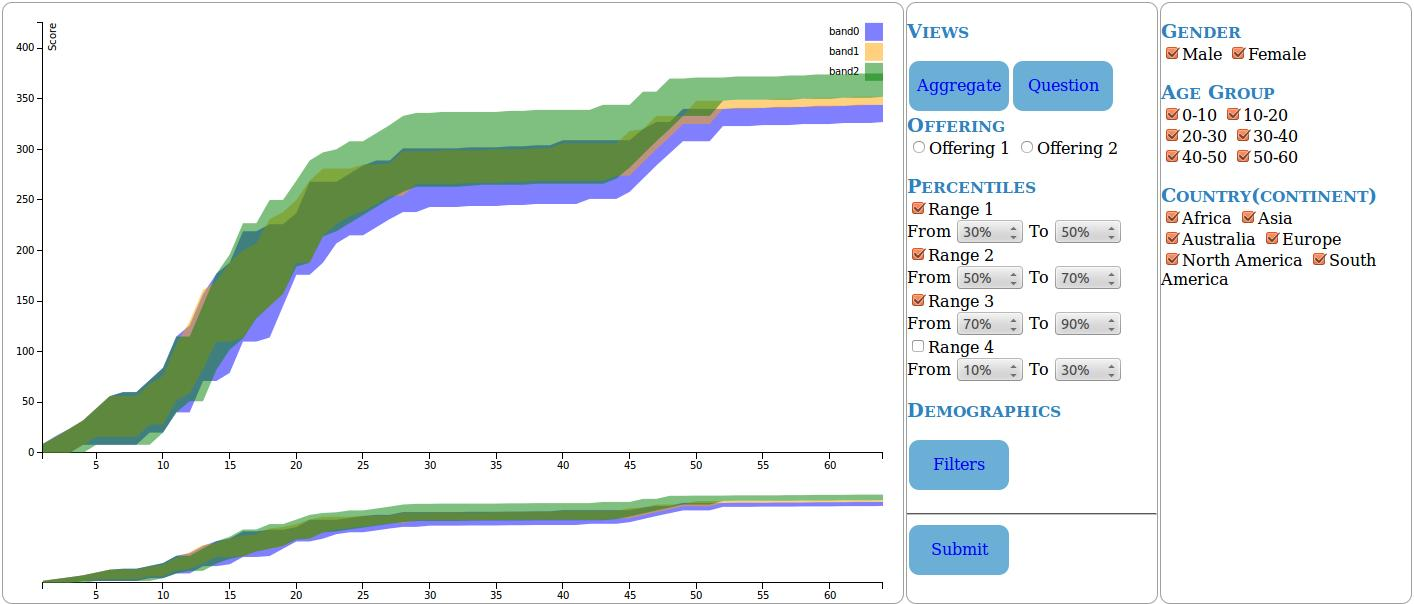
\includegraphics[width=16cm]{Midterm_Final_Aggregate.jpeg}
  \caption{Midterm.}
  }

%% Uncomment below to disable the manuscript note
\renewcommand{\manuscriptnotetxt}{}

%% Copyright space is enabled by default as required by guidelines.
%% It is disabled by the 'review' option or via the following command:
% \nocopyrightspace

\begin{document}
\firstsection{Introduction}
\maketitle

	Often, when course instructors seek information about their in-progress or completed courses, they 
turn to direct data manipulation in software such as Microsoft Excel, Numbers, or Google Docs \cite{ excel, numbers, docs}. 
However, with expansion of educational institutions into course styles such as Massive Open Online 
Courses (MOOCs), the straightforward manipulation of data to find outliers and students who need 
additional assistance becomes too overwhelming for the individual professor to manage in a 
reasonable time frame. 

With courses that enroll tens of thousands of participants in a single offering of a single 
course, it is easy for instructors to be overwhelmed by the sheer amount of data gathered by such 
courses, both in terms of demographics as well as actual results on assignments. Sites such as 
Coursera \cite{coursers} which facilitate the MOOC offerings through interfaces for posting videos as
well as posting, submitting, and grading assignments provide limited interfaces for following a single student---or even a group of students---over the weeks of a course. Nor do they provide any satisfying visualization of the impact of the course elements, despite what is undoubtedly a surfeit of data. 

This project comes in response to the questions of one such professor, who wanted to answer several questions about the programming languages class he had offered twice in the past. Starting with an exploration of the current Coursera data available and their visualizations, moving to working with data (modified for anonymization) generated by actual students, we sought to provide better visualization of the data with several main goals. 

\paragraph{Accessibility}
By far the largest problem with the data in its initial form was accessibility and tractability for 
instructors: though they could get the data into .csv format, it was largely impractical to do calculations
over the data without significant number churning. We provide visualizations with clustering and 
trends so that the data and emerging patterns can be more immediately accessible to the instructors.

\paragraph{Clustering and Comparison}
In addition to visualizing the data in entirety, we allow the instructors to select groups of students, 
through course offering, demographic information, or percentile groups, such that the trends between 
two different student groups can easily be visualized. Providing aggregate data over these groups removes the noise inherent in large datasets, and isolates the important trends. 

\paragraph{Component Impact}
The last important feature we offer to instructors is the ability to isolate the impact of specific components of the course. Whether through the drop-off rate visualized on a time line or the exam questions viewed as a progression through course material, or a best-predictor type view for the final grades, we want instructors to determine which components of their course have the largest and most accurate impact on student retention and success rate (as represented through grades). 

With these goal in mind, we create a visual exploration tool for exploring MOOCs and their data. We 
go over the background and previous work in the next section, explaining the design and methodology
in the following section, and concluding with results and feedback that lead to future work. 

{\bf A note on student privacy. } One of the most delicate aspects of a tool like this is that student data is inherently private. Though one professor did generously give us access to the data from two offerings of his course, much of the demographic data, for example, is not easily available from Coursera due to privacy concerns. Further, tracking students' performance of time may be identifiable in and of itself. For the purposes of this demonstration and writeup we have used the provided data that has been fully anonymized in terms of demographics and slightly tweaked, by the numbers, to ensure further privacy. We provide additional explanations of this in the methodology section.
\section{Background}
	
\subsection{Coursera}

\subsection{D3}
D3.js is a javascript library for manipulating and visualizing data. It takes advantages of SVG, javascript, HTML5 and CSS to provide easy to use and powerful ways to create dynamic visualizations. D3 simplifies data reading, parsing and transformation by providing special support for JSON, geoJSON, CSV and TSV files. It also contains a rich set of templates that greatly simplifies data visualizations, including bar charts, pie charts, scatter plots, etc.

\subsection{Related Research}
We were unable to find previous work looking at courses on the scale of MOOC offerings. 

Previous work seems isolated into a few different areas: analyzing student progress over years of standardized testing, and understanding the progress of students through a single course. The latter is the most similar to what we intend to provide, albeit with different approaches. For example, the work in [1] analyzes students and places them into states, creating a tree-like flow chart of where a student is likely to go next in the course. The overview of educational data mining (EDM) provided in [2] provides a very high-level description of where previous work has gone with respect to evaluating the effectiveness of courses, online material, advising, and so on. Much of this data is either not available to us or is outside the scope of our work, though the clustering techniques we implement are similar in nature to those discussed there. We intend to provide data specifically targeted at the world of MOOCs, where attrition is high, interaction with students is minimal, and the scale of data is too enormous to consider looking at some of the factors involved (like clicks on the course website). Moreover, we would like to provide an overview in a dashboard-like setting for the instructors of the course, to determine utility and effectiveness. 

Outside the scope of EDM, work has gone on in several areas with respect to standardized ?high stakes? exams (e.g. state tests through elementary and high school). Bendinelli and Marder [3] model the data a flow problem, and provide some basis for analysis based on trends and demographic characteristics. However, the data in that paper is severely restricted in scope, and provides minimal analysis at tracking a single individual. Other work looks at the usage data, but not performance [4], and still others are restricted only to looking at progress over several courses [5].

\section{Design and Methods}
	The data we chose to work with was largely data provided by default through Coursera. We have tables of data corresponding to assignments, each of which may be submitted multiple times by a single student. Each submission is tracked with a  timestamp, submission number, and final score. For the midterm and final we have a single submission with timestamp and grade. This aggregate information is at the core of three of our views: {\bf Aggregate View}, {\bf Timescale View} and {\bf
Impact View}

In addition, for each exam we have a breakdown of questions, how many points each was worth, and what percentage of the students correctly answered the question. This information is used to generate
{\bf Exam View} and the comparisons for subviews. 

Finally, we have demographic information for each student. Due to privacy concerns, we generated this data automatically, from the statistics and parameters provided to us based on the actual student data. This random demographic data (gender, age, continent/country and background) is sufficient for us to provide a prototype, though further work would require more accurate data. This data is summarized in the {\bf Demographic View} 

Though all pieces of data are maintained in separate .csv files, the (anonymized) student id allows tracking of student information from one piece of data to the next. Though 65,000 students enrolled in the course, fewer than 27,000 ever watched a video. In the end, we have fewer than 4,000 students who submitted assignments half that number actually completed the course with a passing grade. 

\subsection{Design}
The core of the visualization provided are \emph{views} which switch out the main \emph{graph panel} to isolate different components of the course. To augment the abilities of the graph we provide 
\emph{background computation} to isolate \emph{clusters} of students and \emph{impact} of components. As a fine-grained means of selection, we allow the instructor to superimpose \emph{filters} over the data.


\begin{figure}[htb]
 \centering
 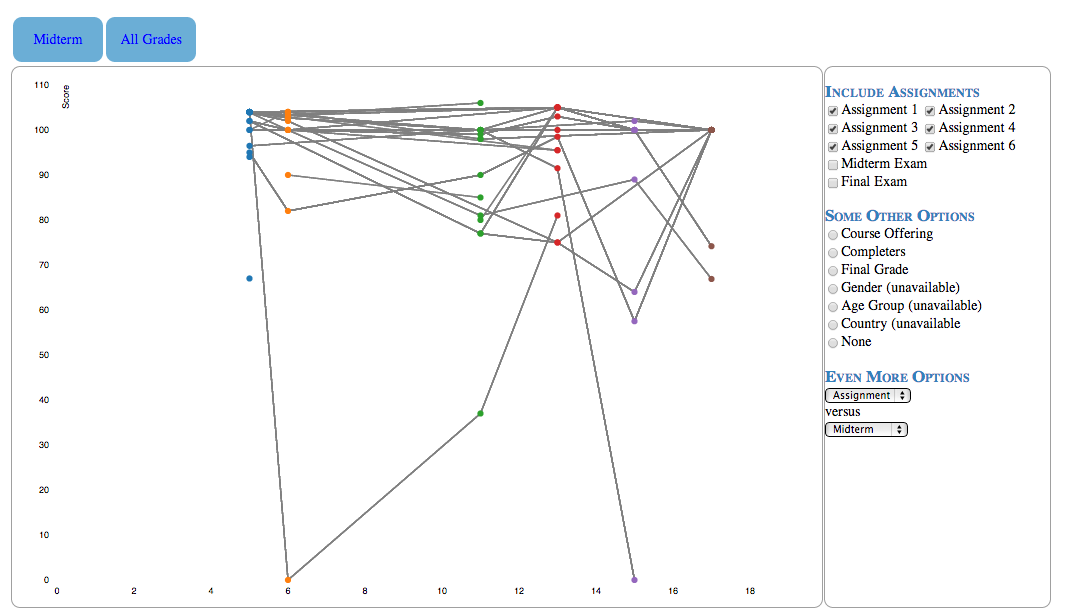
\includegraphics[width=3.5in]{aggregate_stub.png}
 \caption{Aggregate View.}
 \label{fig:aggregate}	
\end{figure}

\paragraph{Aggregate View (see Figure~\ref{fig:aggregate}) }
This view provides a generalized timescale view of the course. Each assignment and exam is represented as a point on the x axis, with grades represented (in percent) on the y axis. This view highlights the retention rate of the class, particularly when clusters are enabled. 


\begin{figure}[htb]
 \centering
 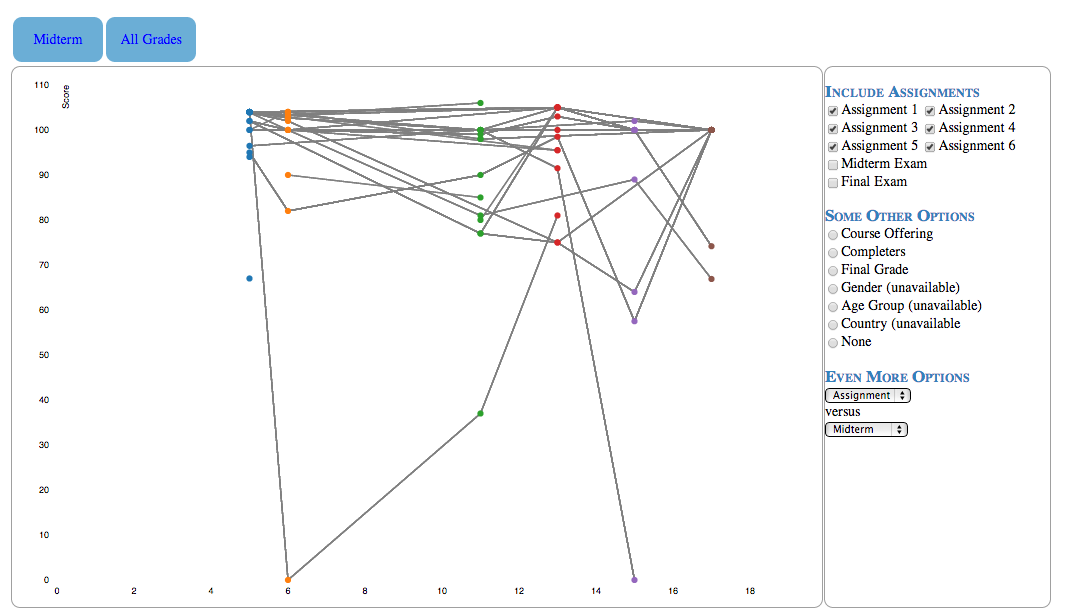
\includegraphics[width=3.5in]{aggregate_stub.png}
 \caption{Timescale View.}
 \label{fig:timescale}	
\end{figure}

\paragraph{Timescale View (see Figure~\ref{fig:timescale}) }
This view provides a zoomed-in view of the assignments and exam scores in relation to the timestamp with which they were submitted. This view originated from a desire to answer the question \emph{do late submitters overall score worse than early submitters?}


\begin{figure}[htb]
 \centering
 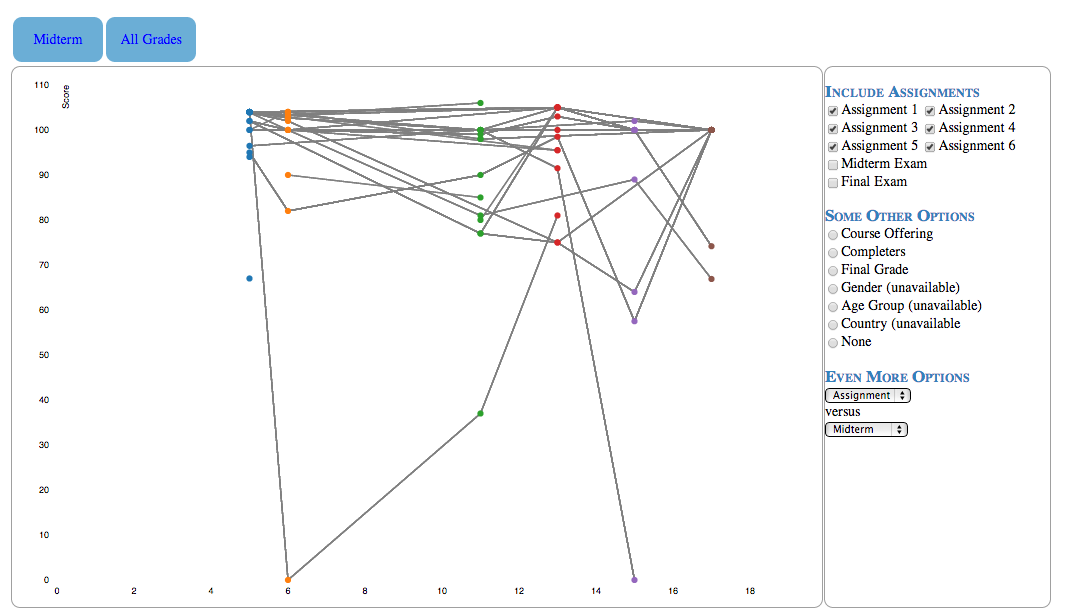
\includegraphics[width=3.5in]{aggregate_stub.png}
 \caption{Impact View.}
 \label{fig:impact}	
\end{figure}

\paragraph{Impact View (see Figure~\ref{fig:impact})}
This view provides a scatterplot reflecting the impact of an assignment or exam on the final grade. Each point is a single student, where the x value is the assignment grade and the y value is the final exam grade. In an ideal world, each assignment would be an equally good predictor of the final grade. When an assignment is a poor predictor, whether a student does well on that exam has little to no impact on the final grade, and we see a randomized scatter plot. When an assignment is a perfect predictor, we see a perfect diagonal formed by the scatter plot. Most assignments fall somewhere between the two.


\begin{figure}[htb]
 \centering
 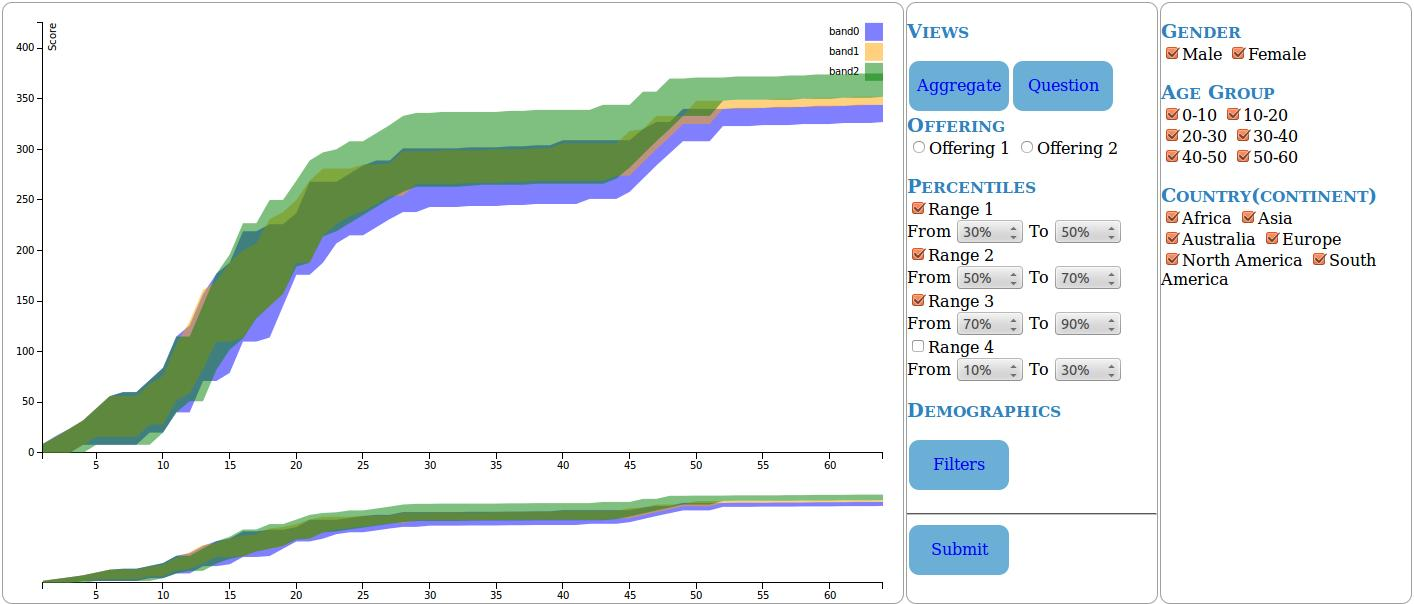
\includegraphics[width=3.5in]{Midterm_Final_Aggregate.jpeg}
 \caption{Comparing Midterm Scores in Aggregate. The exam progresses to the right, and we see the fan-out of scores between percentiles as students diverge in point value. }
\label{fig:exam1}	
\end{figure}

\begin{figure}[htb]
 \centering
 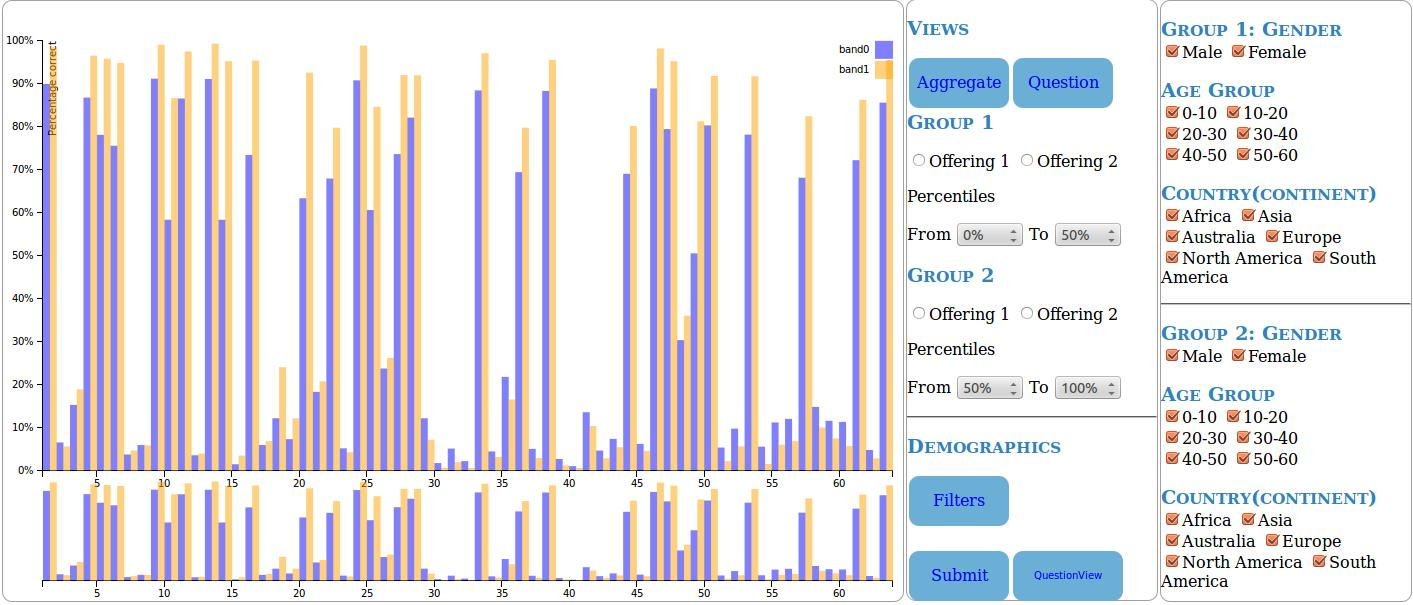
\includegraphics[width=3.5in]{Midterm_Final_Compare.jpeg}
 \caption{Comparing Midterm Scores Across Offerings }
\label{fig:exam2}	
\end{figure}

\begin{figure}[htb]
 \centering
 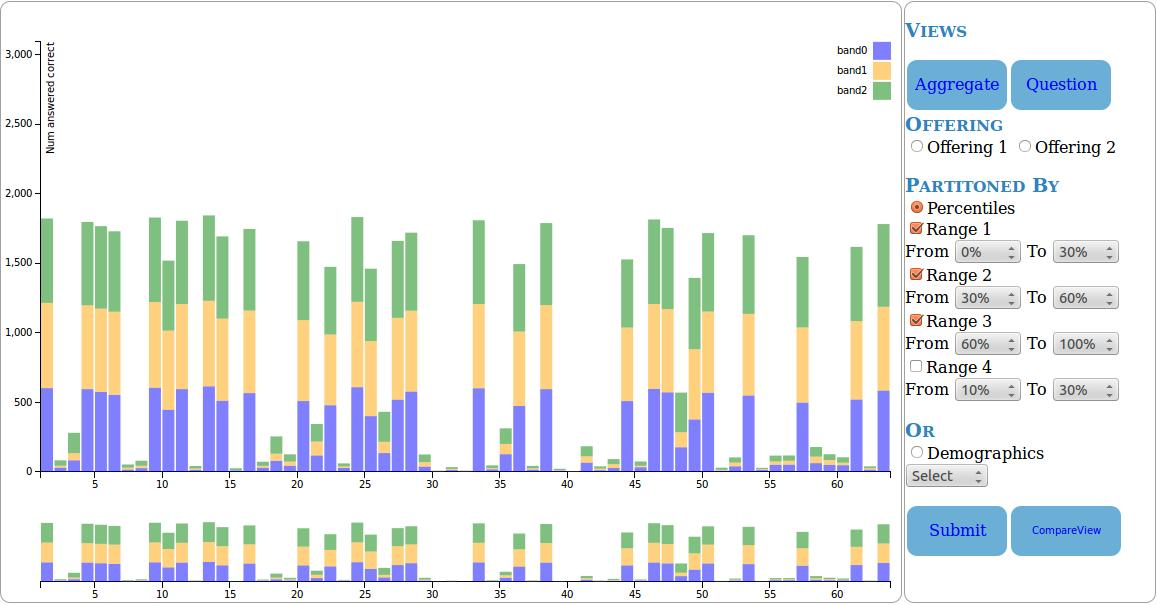
\includegraphics[width=3.5in]{Midterm_Final_Questions.jpeg}
 \caption{Comparing Midterm Questions by Student Percentile. }
\label{fig:exam3}	
\end{figure}

\paragraph{Exam View (see Figure~\ref{fig:exam1})}
TODO


\begin{figure}[htb]
 \centering
 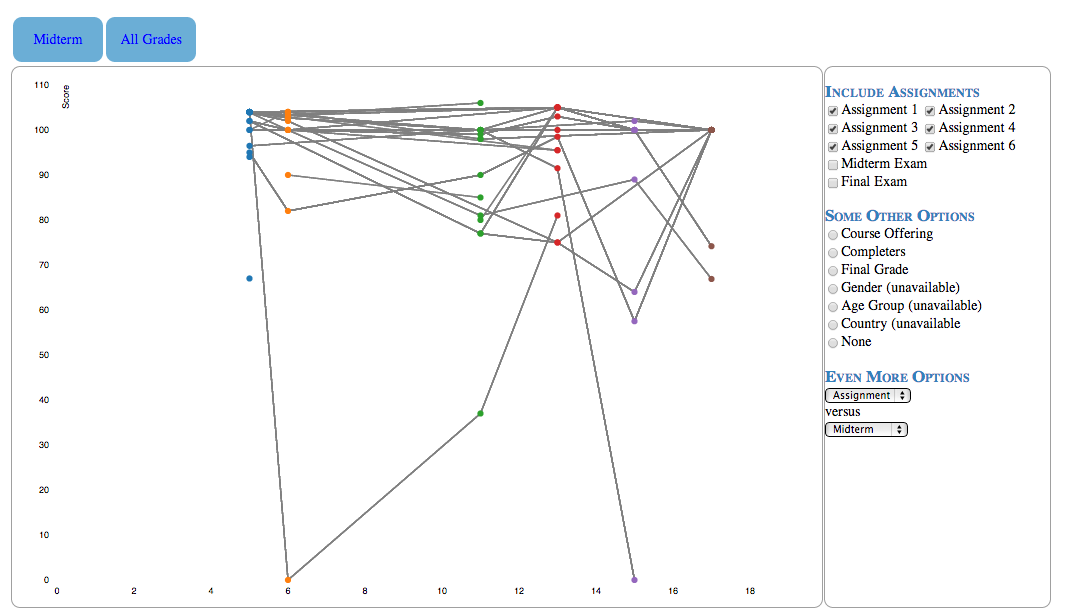
\includegraphics[width=3.5in]{aggregate_stub.png}
 \caption{Demographic View.}
  \label{fig:demo}	
\end{figure}

\paragraph{Demographic View (see Figure~\ref{fig:demo})}
TODO

\subsection{Background Computation}
To save time in loading the actual visualization, some of the computation is done in the background. 

\paragraph{Clustering}
Clusters are precomputed with a script (which must be run prior to the site being launched) and stored in data files for loading 
when requested. Given the quantity of data being processed, this significantly improves the responsiveness for a given page. 
These clusters are computed where the grades of each student (for all time or an exam) are considered a vector, and kmeans 
clustering is applied over the vector, with the distance function being a simple function over each vector pair:
\[  \sqrt{ (a_1-b_1)^2 + (a_2-b_2)^2 .... (a_n-b_n)^2   }\]

\paragraph{Impact}
The course element which most closely predicts the final grade is also precomputed and stored, using the same function above, this time with each assignment being a vector (of which each student is a dimension). However, for the actual display, though we default to the closest predictor (that with the closest distance and/or highest impact), each grade can be displayed without significant computation. Again, pre-computation of the distances saves significantly on load time. 

\section{Results}
	\subsection{Performance}
Our visualization tool is a web-based software that is mostly written in HTML and javascript. Despite the large amount of data we need to process, our tool has a very low response time. We highly optimize the performance of our software by avoiding repeated reading of data (load data only once in the beginning), maximizing references than copying, and reducing asymptotic complexity of filtering functions.

We report the response time of different views in Table~\ref{tab:performance}. Load time indicates time taken to render a page, and filter time indicates time needed to apply some filter options and re-render the page. We ran each experiment for 10 times and took the average. We can see that most of the views are rendered within 50 milliseconds, which is a very reasonable number for a web application. We conducted the experiments on a Dell desktop machine, and all views were loaded instantenously and no significant delay were perceived.

\begin{table}
\begin{tabular}{ | c | c | c | c |}
  \hline
  View & Load Time (ms) & Filter Time (ms) \\ \hline
  Midterm Aggregate & 31.4 & 28.8 \\ \hline
  Midterm Questions & 41.6 & 43.8 \\ \hline
  Midterm Comparison & 44.8 & 47 \\ \hline
\end{tabular}
\caption{Performance table. Shows page load time and filtering time of different views in milliseconds.}
\label{tab:performance}
\end{table}

\section{Discussion}
	
\subsection{Instructor Feedback}
We started the design with the goals of a single professor in mind. He was most interested in a few factors, which we sought to incorporate in our design:
\begin{enumerate}
\item{} Drop-off rate in student retention: how much is normal attrition and how much is caused by the course?
\item{} Cross-offering comparisons: was there significant difference between offerings?
\item{} Performance of female students in the course overall (programming languages is a male-dominated course, in large part. Back-of-the envelope calculations showed that his retention was worse for the female students: was there a reason why?
\end{enumerate}
Though we targeted all three of these questions, we were most successful at answering the first two. Though we allow the instructors to explore trends within demographic groups, the depth of options in exploring the "why" of student retention coupled with demographic variables is not expressed. Further insight into this direction would be possible with stacked filters or pop-up boxes on hover that provide dominant information for a cluster or individual student highlighted. However, this is beyond the scope of the current implementation. 

\subsection{Student Feedback}
Though we initially targeted our design at the instructors of MOOC courses, we found that students 
expressed an equal amount of interest in the data. Both our classmates and other graduate students
who heard about the project were eager to discover whether similar visualizations, perhaps better 
aggregated, could be used to isolate the \emph{difficult weeks} of a course, or which assignments and 
exam questions they were most likely to struggle on. 

\subsection{Additional Feedback}
In presenting an early prototype of our project to a wider community base, via poster, we received plenty of additional feedback. Students and instructors were both intrigued by the retention rate and wanted to ask many more questions about the reasons students left. In addition, many professors were intrigued by the idea of isolating "problem" sections of their exams where they might improve, which drove the development of further exam views. 

Our implementation of a timescale view was driven entirely by responses to the initial prototype, in which a professor confessed she'd always written down the times that assignments and exams were turned in, and had never bothered to plot them to find out if students turned in exams early because they were clueless or brilliant. 

Additional views and data collection schemes were encouraged by nearly everyone, showing that the quantity  and diversity of questions that can be asked in this arena is quite startling. 

Finally, several people at the university level have  expressed interest in incorporating a system such as this into their annual course analytics, incorporating student evaluations of the course and professor's teaching into the mix, but analyzing pure classroom data.
\section{Future Work}
	Though we feel this project represents a solid prototype on the available data, there is a significant amount of work yet to be done in this area. We describe some of the improvements and extensions we would like to make below.

\paragraph{A Wealth of Information}
The amount of data available from the Coursera platform is mind-boggling. Though we used a simple set of grades, timestamps, and demographic data to be able to create this prototype, there is additional data that could provide more insight. Among other things, the use of forum participation, video viewings, and the optional in-video quizzes would provide a rich set of information from which to gauge engagement (frequency of participation) and understanding (frequency of questions and re-watched videos). Other pieces of data such as clicks, and total time to take an exam would be harder to gather, but perhaps more enlightening. 

In addition to supplementing our data with additional information from a single offering or course, we would like to be able to add data from across multiple offerings or multiple courses. With appropriate learning algorithms, we might begin to answer the questions of whether exams are actually helpful, if certain length videos or courses encourage retention and so on. MOOCs are, after all, a large source of rich data to compute over, and Big Data mechanisms applied would provide insights into the utility of certain components. 

\paragraph{Automation and Accessibility}
In addition to providing more data and insights to instructors, we would like to be able to provide easier access. Ideally, we would integrate our tool directly into platforms such as Coursera, though doing so would be a negotiation between development teams. If not that, than at least having a generic auto-upload feature that allows an instructor to upload .csv files and designate columns as demographic, assignment, or exam data would be useful in making the tool more widely available to instructors. As is, the tool is a bit too brittle to enable such usage. 
 
\paragraph{Alternate Viewpoints}
Last of our long-term goals is to look at data sources other than MOOCs. Both students and professors had many suggestions for other uses of the data and resultant visualizations, both for classical classes in a classroom, and for exposing the difficult portions of a course. Exploring these options would provide richer platform. 
\section{Conclusion}
	In conclusion, we present a tool for exploring and visualizing the course data for performance and retention of students in MOOCs. Though the end results poses as many questions as it answers, we believe it is a useful and useable tool for beginning analysis of impact and improvement in course offerings. 


%\begin{figure}[htb]
% \centering
% 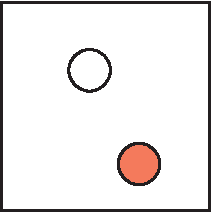
\includegraphics[width=1.5in]{sample}
% \caption{Sample illustration.}
%\end{figure}
%
%
%consequat~\cite{Nielson:1991:TAD}. 
%
\section{References}
[1] Matthew Johnson and Tiffany Barnes. Visualizing Educational Data from Logic Tutors.

[2] Crist�bal Romero and Sebasti�n Ventura. Educational Data Mining: A Review of the
StateoftheArt.

[3]Anthony J. Bendinelli and M. Marder. Visualization of Longitudinal Student Data.

[4] C.Romero, C.Castro, S.Ventura A Moodle Block for Selecting, Visualizing and Mining
Students' Usage Data.

[5].Dana Wortman and Penny Rheingans. Visualizing Trends in Student Performance Across
Computer Science Courses.


%% if specified like this the section will be committed in review mode
\acknowledgments{
The authors wish to heartily thank Dan Grossman, who provided an intro to the Coursera system, as well as a wealth of data to use in our prototype. We also thank the many students and professors who offered input during the development process.}
%
%\bibliographystyle{abbrv}
%%%use following if all content of bibtex file should be shown
%%\nocite{*}
%\bibliography{template}
\end{document}
